\documentclass[9pt]{article}
\usepackage[utf8]{inputenc}
\usepackage{amsmath,amsthm,amsfonts,amssymb,amscd}
\usepackage{multirow,booktabs}
\usepackage{enumitem}
\usepackage{fancyhdr}
\usepackage{mathrsfs}
\usepackage{wrapfig}
\usepackage{setspace}
\usepackage{calc}
\usepackage{multicol}
\usepackage{cancel}
\usepackage[retainorgcmds]{IEEEtrantools}
\usepackage{framed}
\usepackage[most]{tcolorbox}
\usepackage{tikz}
\usepackage{geometry}
\geometry{
	a4paper,
	total={170mm,257mm},
	left=20mm,
	top=20mm,
}
\title{AC currents and RL Circuits}
\author{Aaron G.K.}
\begin{document}
	\maketitle
	\subsection*{AC Currents}
	The current generated by generators and hydroelectric power plants is not a uniform and smooth current - it fluctuates sinusoidally with time. That is purely a result how the flux change is caused. Let's try to mathematically model the current generated by an AC source. \\ \\
	The emf induced is always a result of the change in flux according to Faraday's law. In different cases, the causes of the flux change are different. For instance, during the workings of a generator, the flux change is caused by rotation ($\Delta\theta$); during inductance, the flux change is caused by the changing current which changes the magnetic field($\Delta$I); during motional emf, the flux change is caused by the changing area($\Delta$A).
	\begin{center}
		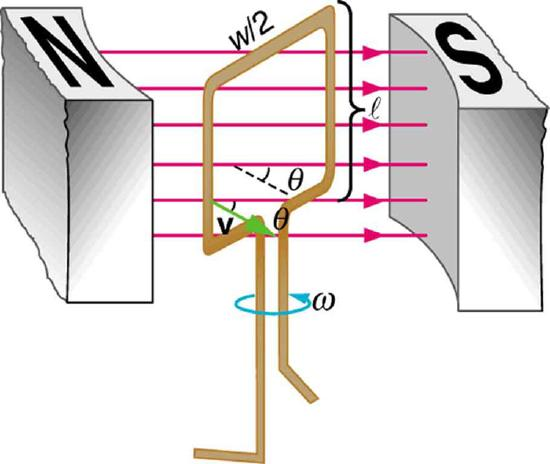
\includegraphics[scale=0.3]{dyn}
	\end{center}
	As we see in our dynamo above, the flux change is caused by the rotation of the coil. We can express the flux change in the flow chart shown below:
	$$\text{rotation}\implies\Delta\theta\implies\text{emf}$$
	If we would like to show our current fluctuates with time, we can express the angular change  in terms of the rate at which its is changing.
	$$\omega=\dfrac{\theta}{t}\implies\theta=\omega t$$
	We know that the flux change here is caused by the change in the angle/orientation of the loop with respects to the magnetic field. 
	$$\Phi=BA\cos\theta\implies\Delta\Phi=BA\cos\Delta\theta\implies\Delta\Phi=BA\cos\omega t$$
	Whenever flux is changing, emf is induced and is given by Faraday's Law:
	$$\mathcal{E}=-N\dfrac{\Delta\Phi}{\Delta t}$$
	We can express using differential calculus as a derivative to study the changes
	$$\mathcal{E}=-N\dfrac{d\Phi}{dt}$$
	$$\mathcal{E}=-N\dfrac{d(BA\cos\omega t)}{dt}$$
	$$\mathcal{E}=NBA\omega\sin(\omega t)$$
	We can see that the function above is a sinusoidal wave that fluctuates with time.
	\begin{center}
		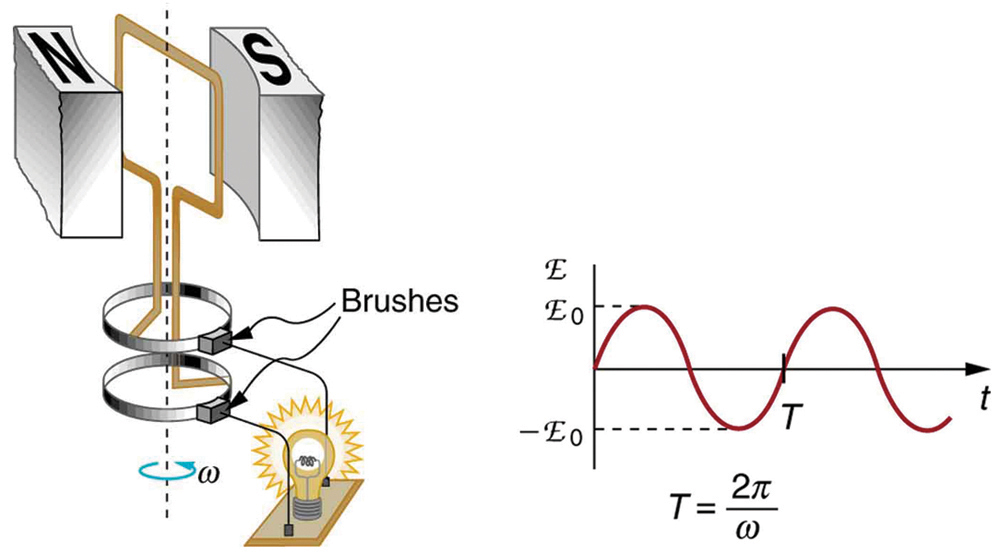
\includegraphics[scale=0.5]{ac.jpg}
	\end{center} 
	\subsection*{RL Circuits}
	RL circuit is a circuit that has resistive and inductive components. We have seen RC circuits in the past and saw that the current and emf in the circuits change exponentially with time. Similarly, we will be looking at RL circuits and our focus will be the impact of inductance in a circuit. Here is a schematic example of a simple RL circuit.
	\begin{center}
		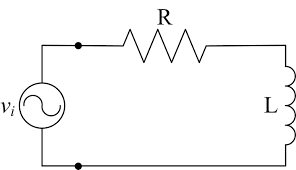
\includegraphics[scale=0.5]{RL}
	\end{center}
	We can see that the emf of the source is divided between the inductor and the resistor since they are connected in series. Thus, the voltage provided by the battery is the sum of the voltages dissipated in the inductor and the resistor.
	$$\mathcal{E}=\mathcal{E}_{\text{IR}}+\mathcal{E}_{\text{L}}$$ 
	$$\mathcal{E}=\text{IR}+\text{L}\dfrac{\varDelta\text{I}}{\varDelta \text{t}}$$ 
	When solving for this equation(this is a differential equation that is similar to the one we had in RC circuits) as we did with RC circuits, we will have two solutions when the current in the circuit is increasing or decreasing.
	\begin{itemize}
		\item When the current is increasing in the circuit, the emf as a function of time is
		$$\mathcal{E}(t)=\mathcal{E}(1-e^{\frac{-\text{Rt}}{\text{L}}})$$
		We can also express the current as a function of time: $I(t)=\dfrac{\mathcal{E}(t)}{R}$.
		$$I(t)=\dfrac{\mathcal{E}(t)}{R}=\dfrac{\mathcal{E}(1-e^{\frac{-\text{Rt}}{\text{L}}})}{R}$$
		\item When the current is decreasing in the circuit, the emf as a function of time is
		$$\mathcal{E}(t)=\mathcal{E}e^{\frac{-\text{Rt}}{\text{L}}}$$
		As shown above, we can express the current as a function of time and it is
		$$\mathcal{E}(t)=\dfrac{\mathcal{E}e^{\frac{-\text{Rt}}{\text{L}}}}{R}$$
	\end{itemize}
	We define the quantity inductive(characteristic) time constant as $\tau_\text{L}=\dfrac{\text{L}}{\text{R}}$. \\ \\
	$$V_L(t)=-\varepsilon e^{\frac{-t}{\tau_L}}$$
	In case of the induced voltage as a result of inductance($V_L$), we have seen that it is directly proportional to the time rate of change of current. That means, it will have its maximum value immediately after the switch is turned on in the circuit and its value decreases along with time. When the current is maximum($\frac{\varepsilon}{R}$), the induced voltage becomes 0.
	The inductive time constant tells us how fast the voltage decays and also how fast the current exponentially increases. It is an indicative measure of rapid changes in the circuit. The energy stored in an RL circuit is given by the following:
	$$E=\frac{1}{2}LI^2$$
\end{document}